\setmainfont{Noto Serif}
\setsansfont{Noto Sans}
\setmonofont{Noto Sans Mono}
\setstretch{1.35}

\section{Химический обмен в магнитном резонансе}
1C. Изобразите трансформацию спектра ЭПР при увеличении скорости химической реакции: 
\text{H} + $\text{H}_2$ $\rightleftarrows$ $\text{H}_3$ (циклическая система).
\par
\begin{wrapfigure}{r}{51mm} %this figure will be at the right
    \centering
    \vspace{-0mm}
    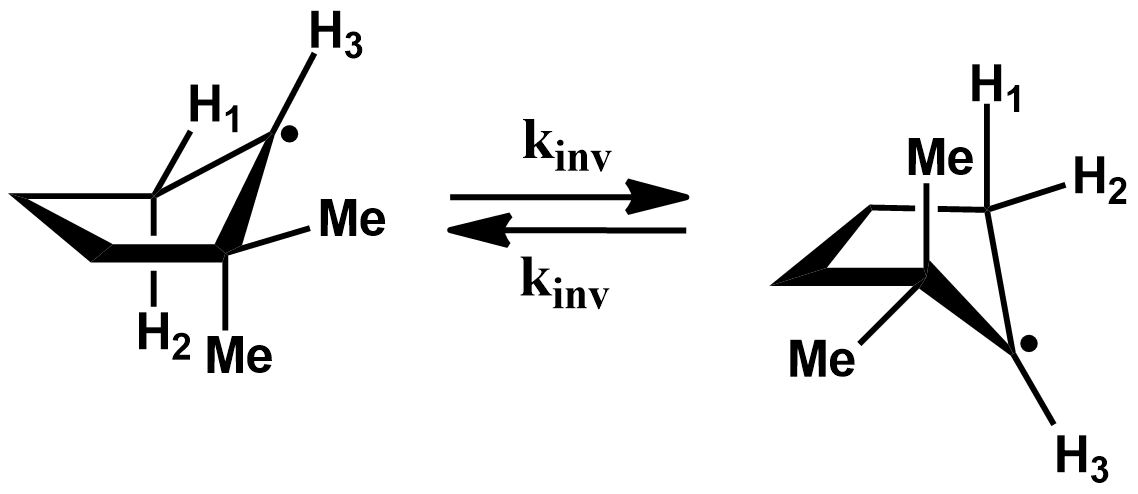
\includegraphics[width=45mm]{images/Fig_2_8_2.png}
    \vspace{-4mm}
\end{wrapfigure}
2К. 2,2-диметилциклопентильный радикал имеет две инверсные конформации, приведенные на рисунке. Константа СТВ протона в третьем положении равна 15~Гс, а протонов $\text{CH}_2$-фрагмента 20 Гс и 10~Гс в~экваториальном и аксиальном положениях, соответственно. Постройте спектр ЭПР данного радикала для случаев: (1)~отсутствия обмена экваториальных и аксиальных протонов $\text{H}_1$ $\rightleftarrows$ $\text{H}_2$, (2)~медленного обмена при $k_{inv}$ $\ll$ СТВ, (3)~быстрого обмена при $k_{inv}$ $\gg$ СТВ.
\par
\begin{wrapfigure}{r}{51mm} %this figure will be at the right
    \centering
    \vspace{-0mm}
    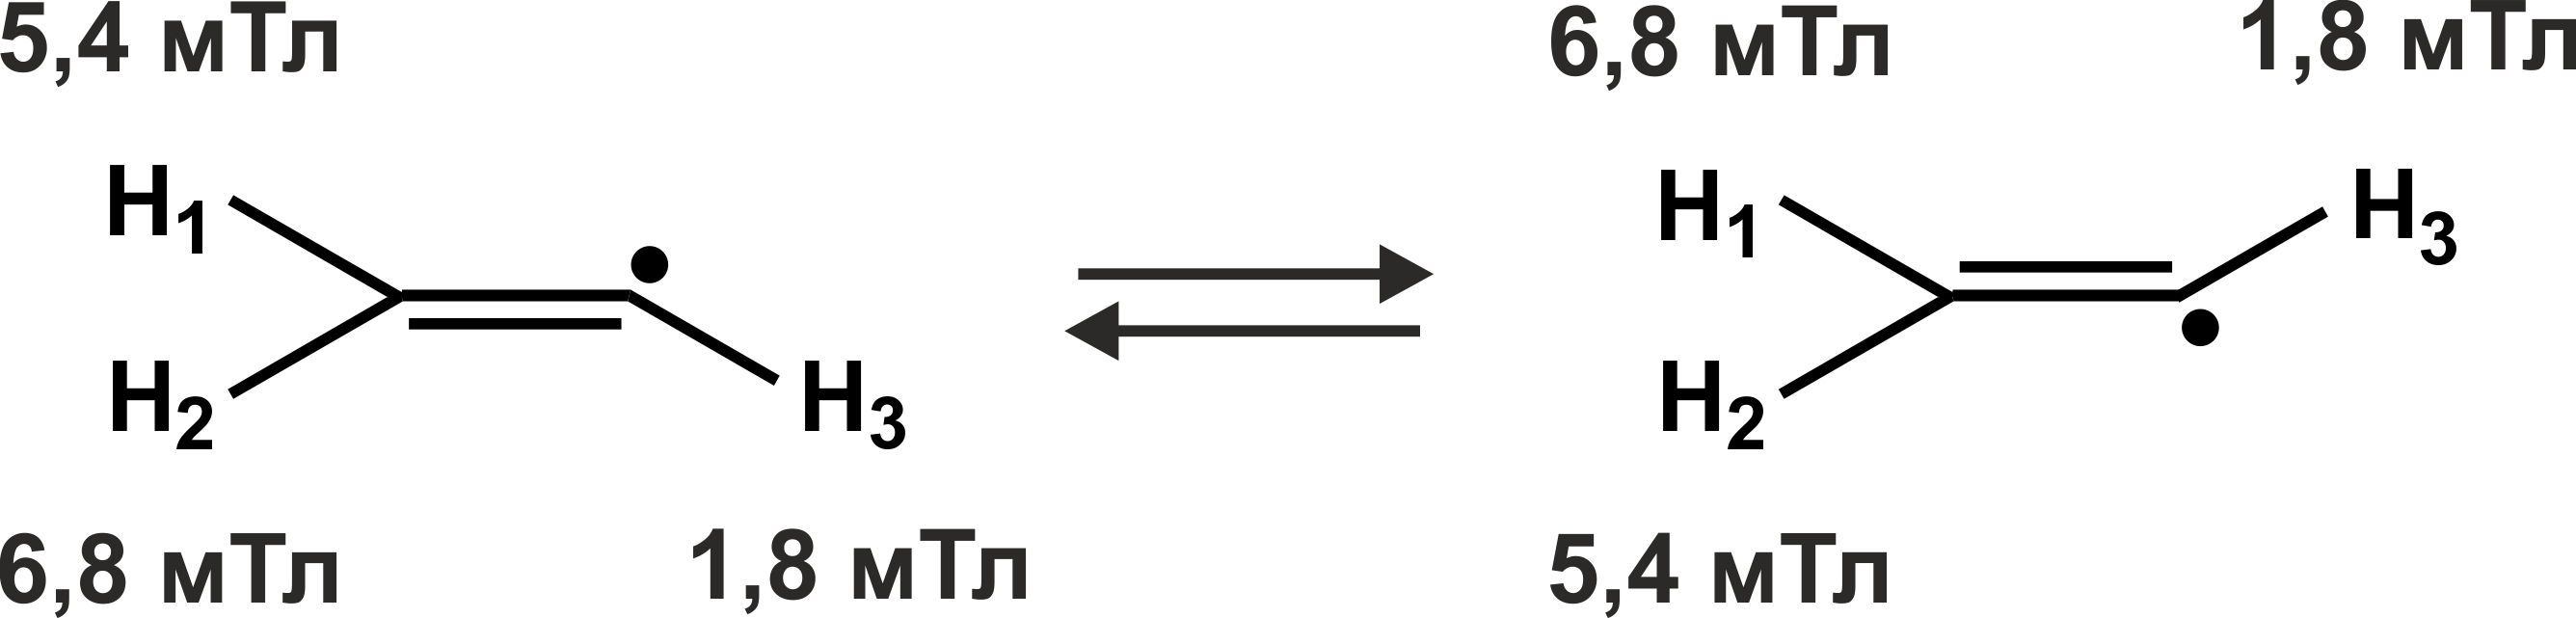
\includegraphics[width=51mm]{images/Fig_2_8_4.png}
    \vspace{-4mm}
\end{wrapfigure}
3К. Опишите изменения в спектре ЭПР винильного радикала, происходящие при увеличении скорости превращения его таутомеров. Константы СТВ приведены на рисунке справа. В частности нарисуйте ЭПР спектр, наблюдаемый при низкой температуре в жесткой матрице, спектр, наблюдаемый при промежуточной температуре, а также ЭПР спектр, регистрируемый в невязкой жидкости.
\par
4С. В кристаллах алмаза наблюдаются дефекты с одним неспаренным электроном, содержащие азот следующего типа: $\text{N}_1-\text{C}-\text{N}_2$. Неспаренный электрон взаимодействует с ядрами азота, имеющими константу $a_1$ = 30 Гс и $a_2$ = 5 Гс, соответственно. Причем $a_1$ и $a_2$ могут иметь одинаковые знаки и различные знаки, могут быть как положительными, так и отрицательными. При повышении температуры происходит обмен ядрами азота: $\text{N}_1-\text{C}-\text{N}_2$ $\rightleftarrows$ $\text{N}_2-\text{C}-\text{N}_1$. Опишите картину процесса в двух случаях, различающихся знаками одной из~констант СТВ: (1) $a_1$ = 30 Гс и $a_2$ = +5 Гс, (2) $a_1$ = 30 Гс и $a_2$ = $-$5 Гс.
\par
5С. Определите изменение спектров ЯМР, полученных на ядрах $^{19}\text{F}$ и $^{31}\text{P}$, для молекулы $\text{PF}_5$ при увеличении скорости: (1) внутримолекулярного обмена всех атомов фтора, (2) межмолекулярного обмена аксиальных атомов фтора. Константы спин-спинового взаимодействия уменьшаются в следующем порядке: $J(\text{P}-\text{F}_\text{a})$ $>$ $J(\text{P}-\text{F}_\text{э})$ $>$ $J(\text{F}_\text{э}-\text{F}_\text{a})$.
\par
\begin{wrapfigure}{r}{33mm} %this figure will be at the right
    \centering
    \vspace{0.7mm}
    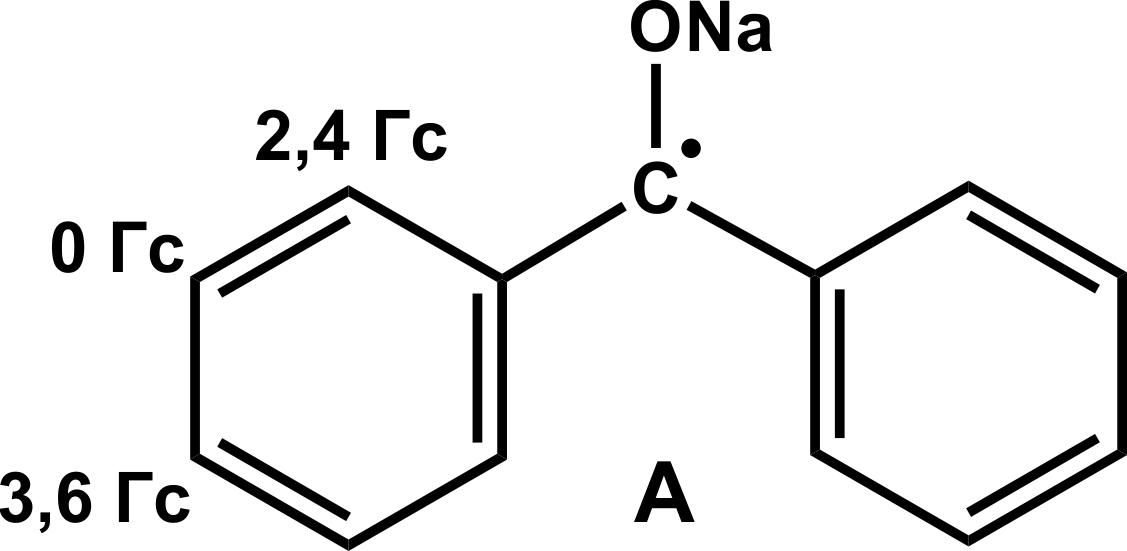
\includegraphics[width=33mm]{images/Fig_2_8_8.png}
    \vspace{0mm}
\end{wrapfigure}
6К. ЭПР спектр разбавленного раствора кетила бензофенона натрия, соединение А, в 1,2-диметок-сиэтане содержит 52 линии. Константы СТВ в анион-радикале бензофенона приведены на рисунке. Объясните, чем может быть вызвано такое количество линий в спектре ЭПР данного кетила. В присутствии избытка бензофенона в растворе также протекает реакция:
\[\text{NaO}\boldsymbol{\dot{\text{C}}}(\text{C}_6\text{H}_5)_2 + \text{O}\text{C}(\text{C}_6\text{H}_5)_2 = \text{O}\text{C}(\text{C}_6\text{H}_5)_2 + \text{NaO}\boldsymbol{\dot{\text{C}}}(\text{C}_6\text{H}_5)_2\]
С помощью ЭПР спектроскопии возможно установить протекает ли данная реакция (1) в результате переноса атома натрия или (2) в результате некоррелированного переноса электронов и катионов натрия $\text{Na}^+$. Как будет выглядеть спектр ЭПР смеси при достаточной высокой для протекания быстрого обмена концентрации бензофенона в указанных двух случаях. Кетилами называют анион-радикалы общей формулы $\text{R}_2 \boldsymbol{\dot{\text{C}}}-\text{O}^-$ и их соли, то есть продукты одноэлектронного восстановления кетонов.
\par